% ==============================================================================
% CHAPTER 5 — Support Vector Machines
% ==============================================================================
\chapter{Support Vector Machines}\label{ch:svm}

\begin{intuition}[title=\textbf{Chapter Overview}]
Support Vector Machines find the hyperplane that separates classes with the \emph{largest margin}. This geometric principle leads to a convex optimisation problem with strong theoretical guarantees. This chapter derives the hard-margin and soft-margin formulations, introduces the dual problem and KKT conditions, and presents the kernel trick for nonlinear classification.
\end{intuition}

% ==============================================================================
\section{Maximum Margin Classifier}
% ==============================================================================

\subsection{Setup and Geometric Motivation}

\begin{definition}[Linear Classifier]
Given training data $\{(\bm{x}_i, y_i)\}_{i=1}^{n}$ with $\bm{x}_i \in \R^p$ and $y_i \in \{-1, +1\}$, a linear classifier predicts
\[
    \hat{y} = \sign(\bm{w}^\top\bm{x} + b),
\]
where $\bm{w} \in \R^p$ is the weight vector and $b \in \R$ the bias.
\end{definition}

\begin{definition}[Functional and Geometric Margin]
The \emph{functional margin} of sample $(\bm{x}_i, y_i)$ is $\hat{\gamma}_i = y_i(\bm{w}^\top\bm{x}_i + b)$. The \emph{geometric margin} is the signed distance to the hyperplane:
\[
    \gamma_i = \frac{y_i(\bm{w}^\top\bm{x}_i + b)}{\norm{\bm{w}}}.
\]
The margin of the dataset is $\gamma = \min_i \gamma_i$. A positive functional margin indicates correct classification.
\end{definition}

\begin{lemma}[Distance to a Hyperplane]
For a hyperplane $H = \{\bm{x} : \bm{w}^\top\bm{x} + b = 0\}$, the Euclidean distance from any point $\bm{x}_0$ to $H$ is
\[
    d(\bm{x}_0, H) = \frac{|\bm{w}^\top\bm{x}_0 + b|}{\norm{\bm{w}}}.
\]
\end{lemma}

\begin{proof}
Any point on the hyperplane satisfies $\bm{w}^\top\bm{x} + b = 0$. The projection of $\bm{x}_0$ onto $H$ along the normal $\bm{w}/\norm{\bm{w}}$ gives $\bm{x}_0 - \frac{\bm{w}^\top\bm{x}_0+b}{\norm{\bm{w}}^2}\bm{w}$. The distance is $\norm{\frac{\bm{w}^\top\bm{x}_0+b}{\norm{\bm{w}}^2}\bm{w}} = \frac{|\bm{w}^\top\bm{x}_0+b|}{\norm{\bm{w}}}$.
\end{proof}

\begin{center}
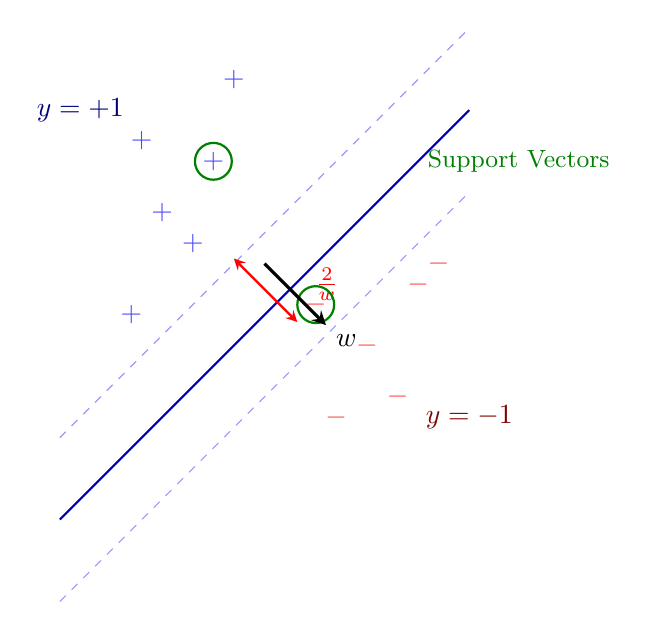
\begin{tikzpicture}[scale=1.3, >=stealth]
    % Hyperplane
    \draw[thick, blue!70!black] (-0.5,-1.5) -- (3.5,2.5);
    % Margin boundaries
    \draw[dashed, blue!40] (-0.5,-0.7) -- (3.5,3.3);
    \draw[dashed, blue!40] (-0.5,-2.3) -- (3.5,1.7);
    % Margin arrow
    \draw[<->, thick, red] (1.2,1.05) -- (1.82,0.43);
    \node[red, right] at (1.9,0.8) {$\frac{2}{\norm{\bm{w}}}$};
    % Positive class
    \foreach \x/\y in {0.2/0.5, 0.5/1.5, 1.0/2.0, 0.3/2.2, 1.2/2.8, 0.8/1.2}{
        \node[blue!70, font=\bfseries] at (\x,\y) {$+$};
    }
    % Negative class
    \foreach \x/\y in {2.5/0.2, 3.0/0.8, 2.8/-0.3, 3.2/1.0, 2.2/-0.5, 2.0/0.6}{
        \node[red!70, font=\bfseries] at (\x,\y) {$-$};
    }
    % Support vectors (circled)
    \draw[green!50!black, thick] (1.0,2.0) circle (0.18);
    \draw[green!50!black, thick] (2.0,0.6) circle (0.18);
    % Normal vector
    \draw[->, very thick, black] (1.5,1.0) -- (2.1,0.4);
    \node[black] at (2.3,0.25) {$\bm{w}$};
    % Labels
    \node[blue!50!black] at (-0.3,2.5) {$y=+1$};
    \node[red!50!black] at (3.5,-0.5) {$y=-1$};
    \node[green!50!black, right] at (3.0,2.0) {\small Support Vectors};
\end{tikzpicture}
\end{center}

% ==============================================================================
\section{Hard-Margin SVM}
% ==============================================================================

\begin{definition}[Hard-Margin Primal Problem]
Assuming the data is linearly separable, the maximum-margin hyperplane solves
\[
    \min_{\bm{w}, b}\; \frac{1}{2}\norm{\bm{w}}^2
    \qquad \text{s.t.}\quad y_i(\bm{w}^\top\bm{x}_i + b) \geq 1, \;\; i = 1,\ldots,n.
\]
\end{definition}

\begin{theorem}[Margin Width]
The margin of the optimal hyperplane is $\gamma^* = \frac{2}{\norm{\bm{w}^*}}$. The constraints $y_i(\bm{w}^\top\bm{x}_i+b) \geq 1$ normalise the functional margin to $1$, so the geometric margin equals $1/\norm{\bm{w}}$ on each side.
\end{theorem}

\begin{remark}
Maximising $\frac{2}{\norm{\bm{w}}}$ is equivalent to minimising $\frac{1}{2}\norm{\bm{w}}^2$, which is a convex quadratic objective with linear constraints --- a Quadratic Program (QP). The $\frac{1}{2}$ is for algebraic convenience and does not affect the solution.
\end{remark}

\begin{proposition}[Uniqueness]
Since the objective is strictly convex and the constraints are linear (hence convex), the hard-margin SVM has a unique solution $(\bm{w}^*,b^*)$ whenever the feasible set is non-empty (data is linearly separable).
\end{proposition}

% ==============================================================================
\section{Soft-Margin SVM}
% ==============================================================================

\begin{definition}[Soft-Margin Primal Problem]
When data is not perfectly separable, introduce slack variables $\xi_i \geq 0$:
\[
    \min_{\bm{w}, b, \bm{\xi}}\; \frac{1}{2}\norm{\bm{w}}^2 + C\sum_{i=1}^{n}\xi_i
    \qquad \text{s.t.}\quad
    \begin{cases}
        y_i(\bm{w}^\top\bm{x}_i + b) \geq 1 - \xi_i,\\
        \xi_i \geq 0, \quad i = 1,\ldots,n.
    \end{cases}
\]
The parameter $C > 0$ trades off margin width against training errors.
\end{definition}

\begin{proposition}[Interpretation of $\xi_i$]
\begin{itemize}
    \item $\xi_i = 0$: point $i$ is correctly classified and outside the margin.
    \item $0 < \xi_i < 1$: correctly classified but inside the margin.
    \item $\xi_i = 1$: on the decision boundary.
    \item $\xi_i > 1$: misclassified.
\end{itemize}
The sum $\sum_i \xi_i$ is an upper bound on the number of training errors.
\end{proposition}

\begin{warning}[title=\textbf{Role of $C$}]
$C \to \infty$ recovers the hard-margin SVM (no violations allowed). Small $C$ permits more margin violations, producing a wider margin but more misclassifications. The optimal $C$ is typically selected via cross-validation over a logarithmic grid (e.g.\ $C \in \{10^{-3}, 10^{-2}, \ldots, 10^{3}\}$).
\end{warning}

\begin{proposition}[Hinge Loss Formulation]
The soft-margin SVM is equivalent to the unconstrained problem
\[
    \min_{\bm{w},b}\;\frac{1}{2}\norm{\bm{w}}^2 + C\sum_{i=1}^{n}\max\bigl(0,\, 1-y_i(\bm{w}^\top\bm{x}_i+b)\bigr),
\]
where $\ell_{\text{hinge}}(z) = \max(0, 1-z)$ is the \emph{hinge loss}.
\end{proposition}

% ==============================================================================
\section{Dual Formulation and KKT Conditions}
% ==============================================================================

\subsection{Lagrangian and Dual}

\begin{theorem}[Dual Problem of the Soft-Margin SVM]\label{thm:svm-dual}
The Lagrangian dual of the soft-margin SVM is
\[
    \max_{\bm{\alpha}}\; \sum_{i=1}^{n}\alpha_i - \frac{1}{2}\sum_{i,j}\alpha_i\alpha_j y_i y_j \inner{\bm{x}_i}{\bm{x}_j}
    \qquad \text{s.t.}\quad
    \begin{cases}
        0 \leq \alpha_i \leq C, \quad \forall\, i, \\
        \sum_{i=1}^{n}\alpha_i y_i = 0.
    \end{cases}
\]
\end{theorem}

\begin{proof}
Form the Lagrangian with multipliers $\alpha_i \geq 0$ (for the margin constraints) and $\mu_i \geq 0$ (for $\xi_i \geq 0$):
\[
    \mathcal{L} = \frac{1}{2}\norm{\bm{w}}^2 + C\sum_i\xi_i
    - \sum_i\alpha_i[y_i(\bm{w}^\top\bm{x}_i+b)-1+\xi_i]
    - \sum_i\mu_i\xi_i.
\]
Setting partial derivatives to zero:
\begin{align}
    \frac{\partial\mathcal{L}}{\partial\bm{w}} &= \bm{w} - \sum_i\alpha_i y_i\bm{x}_i = \bm{0}
    \;\Longrightarrow\; \bm{w} = \sum_i\alpha_i y_i\bm{x}_i, \label{eq:w-dual}\\
    \frac{\partial\mathcal{L}}{\partial b} &= -\sum_i\alpha_i y_i = 0, \label{eq:b-dual}\\
    \frac{\partial\mathcal{L}}{\partial\xi_i} &= C - \alpha_i - \mu_i = 0
    \;\Longrightarrow\; \alpha_i \leq C. \label{eq:xi-dual}
\end{align}
Substituting \eqref{eq:w-dual}--\eqref{eq:xi-dual} back into $\mathcal{L}$ eliminates $\bm{w}$, $b$, and $\bm{\xi}$:
\begin{align*}
    \mathcal{L} &= \frac{1}{2}\sum_{i,j}\alpha_i\alpha_j y_i y_j\inner{\bm{x}_i}{\bm{x}_j} - \sum_{i,j}\alpha_i\alpha_j y_i y_j\inner{\bm{x}_i}{\bm{x}_j} + \sum_i\alpha_i\\
    &= \sum_i\alpha_i - \frac{1}{2}\sum_{i,j}\alpha_i\alpha_j y_i y_j\inner{\bm{x}_i}{\bm{x}_j},
\end{align*}
yielding the dual objective.
\end{proof}

\begin{remark}
The dual problem is a concave QP with box constraints ($0 \leq \alpha_i \leq C$) and one linear equality constraint ($\sum \alpha_i y_i = 0$). The SMO (Sequential Minimal Optimisation) algorithm by Platt (1998) solves it efficiently by iteratively optimising pairs of $\alpha_i$ values.
\end{remark}

\subsection{KKT Conditions}

\begin{theorem}[KKT Conditions for SVM]
At optimality, the following conditions hold for all $i$:
\begin{enumerate}
    \item \textbf{Primal feasibility:} $y_i(\bm{w}^\top\bm{x}_i+b) \geq 1-\xi_i$, $\xi_i \geq 0$.
    \item \textbf{Dual feasibility:} $0 \leq \alpha_i \leq C$.
    \item \textbf{Complementary slackness:}
    \[
        \alpha_i[y_i(\bm{w}^\top\bm{x}_i+b)-1+\xi_i] = 0,
        \qquad (C-\alpha_i)\xi_i = 0.
    \]
    \item \textbf{Stationarity:} $\bm{w} = \sum_i \alpha_i y_i \bm{x}_i$ and $\sum_i \alpha_i y_i = 0$.
\end{enumerate}
\end{theorem}

\begin{proposition}[Classification of Training Points via KKT]
The KKT conditions partition training points into three categories:
\begin{itemize}
    \item $\alpha_i = 0$: non-support vector, lies outside the margin, $\xi_i = 0$.
    \item $0 < \alpha_i < C$: support vector on the margin, $\xi_i = 0$, $y_i(\bm{w}^\top\bm{x}_i+b) = 1$.
    \item $\alpha_i = C$: support vector inside or on wrong side of margin, $\xi_i > 0$.
\end{itemize}
\end{proposition}

\begin{proposition}[Support Vectors]
A training point $(\bm{x}_i, y_i)$ is a \emph{support vector} if and only if $\alpha_i > 0$. The optimal $\bm{w}$ depends only on support vectors via $\bm{w} = \sum_{i:\alpha_i>0}\alpha_i y_i\bm{x}_i$.
\end{proposition}

\begin{proposition}[Recovery of $b$]
For any support vector with $0 < \alpha_i < C$ (so $\xi_i = 0$ by the second complementary slackness condition):
\[
    b = y_i - \bm{w}^\top\bm{x}_i = y_i - \sum_{j:\alpha_j>0}\alpha_j y_j\inner{\bm{x}_j}{\bm{x}_i}.
\]
In practice, average over all such support vectors for numerical stability.
\end{proposition}

% ==============================================================================
\section{Kernel Trick --- Introduction}
% ==============================================================================

\begin{definition}[Kernel Function]
A function $K : \R^p \times \R^p \to \R$ is a (positive definite) kernel if there exists a feature map $\phi : \R^p \to \mathcal{H}$ into a Hilbert space such that
\[
    K(\bm{x}, \bm{x}') = \inner{\phi(\bm{x})}{\phi(\bm{x}')}_{\mathcal{H}}.
\]
\end{definition}

\begin{theorem}[Kernelised SVM]
In the dual, the data appear only via inner products $\inner{\bm{x}_i}{\bm{x}_j}$. Replacing these by $K(\bm{x}_i, \bm{x}_j)$ implicitly maps data to a higher-dimensional (possibly infinite) space without ever computing $\phi(\bm{x})$. The decision function becomes
\[
    f(\bm{x}) = \sum_{i=1}^{n}\alpha_i y_i K(\bm{x}_i, \bm{x}) + b.
\]
\end{theorem}

\begin{example}[Common Kernels]
\begin{itemize}
    \item \textbf{Linear:} $K(\bm{x},\bm{x}') = \bm{x}^\top\bm{x}'$.
    \item \textbf{Polynomial:} $K(\bm{x},\bm{x}') = (\bm{x}^\top\bm{x}' + c)^d$, $c \geq 0$, $d \in \mathbb{N}$.
    \item \textbf{RBF (Gaussian):} $K(\bm{x},\bm{x}') = \exp\!\bigl(-\gamma\norm{\bm{x}-\bm{x}'}^2\bigr)$, $\gamma = \frac{1}{2\sigma^2} > 0$.
    \item \textbf{Sigmoid:} $K(\bm{x},\bm{x}') = \tanh(\kappa\,\bm{x}^\top\bm{x}' + c)$ (valid only for certain $\kappa, c$).
\end{itemize}
\end{example}

\begin{lemma}[Mercer's Condition]
A continuous symmetric function $K$ is a valid kernel if and only if the Gram matrix $[K(\bm{x}_i,\bm{x}_j)]_{i,j}$ is positive semi-definite for any finite set $\{\bm{x}_1,\ldots,\bm{x}_n\}$.
\end{lemma}

\begin{proposition}[RBF Feature Space]
The RBF kernel corresponds to an infinite-dimensional feature map. Its Taylor expansion $e^{-\gamma\norm{\bm{x}-\bm{x}'}^2} = e^{-\gamma\norm{\bm{x}}^2}e^{-\gamma\norm{\bm{x}'}^2}\sum_{k=0}^{\infty}\frac{(2\gamma)^k}{k!}(\bm{x}^\top\bm{x}')^k$ shows it is a weighted sum of polynomial kernels of all degrees.
\end{proposition}

\begin{bestpractice}[title=\textbf{Choosing the Kernel}]
\begin{itemize}
    \item Start with a linear kernel; it is fast and interpretable.
    \item Use RBF when the decision boundary is nonlinear; tune $\gamma = 1/(2\sigma^2)$ and $C$ via grid search.
    \item Polynomial kernels are useful when feature interactions of a known degree matter.
    \item Always standardise features before training an SVM.
    \item scikit-learn default for \texttt{SVC}: RBF kernel with $\gamma = 1/(p\cdot\Var(X))$ (\texttt{gamma='scale'}).
\end{itemize}
\end{bestpractice}

% ==============================================================================
\section{Implementation in Python}
% ==============================================================================

\subsection{SVM with scikit-learn}

\begin{codeblock}[title=\textbf{SVM Classification with scikit-learn}]
\begin{minted}{python}
import numpy as np
from sklearn.datasets import make_classification
from sklearn.model_selection import train_test_split, GridSearchCV
from sklearn.preprocessing import StandardScaler
from sklearn.svm import SVC
from sklearn.metrics import accuracy_score, classification_report

X, y = make_classification(n_samples=300, n_features=2,
                           n_redundant=0, n_clusters_per_class=1,
                           random_state=42)
X_train, X_test, y_train, y_test = train_test_split(
    X, y, test_size=0.3, random_state=42)

scaler = StandardScaler().fit(X_train)
X_tr = scaler.transform(X_train)
X_te = scaler.transform(X_test)

# Grid search over C and kernel
param_grid = {
    "C": [0.1, 1, 10, 100],
    "kernel": ["linear", "rbf"],
    "gamma": ["scale", "auto"],
}
grid = GridSearchCV(SVC(), param_grid, cv=5, scoring="accuracy")
grid.fit(X_tr, y_train)

print(f"Best params: {grid.best_params_}")
print(f"CV accuracy: {grid.best_score_:.3f}")
print(f"Test accuracy: {accuracy_score(y_test, grid.predict(X_te)):.3f}")

# Number of support vectors
best_svm = grid.best_estimator_
print(f"Support vectors per class: {best_svm.n_support_}")
print(f"Total support vectors: {sum(best_svm.n_support_)} / {len(y_train)}")
\end{minted}
\end{codeblock}

\begin{codeoutput}
\begin{minted}{text}
Best params: {'C': 1, 'gamma': 'scale', 'kernel': 'rbf'}
CV accuracy: 0.919
Test accuracy: 0.922
Support vectors per class: [32 35]
Total support vectors: 67 / 210
\end{minted}
\end{codeoutput}

\subsection{SVM from Scratch (Simplified)}

\begin{codeblock}[title=\textbf{Soft-Margin SVM via Subgradient Descent}]
\begin{minted}{python}
import numpy as np

def svm_sgd(X, y, C=1.0, eta0=0.01, n_iter=1000):
    """Train a linear SVM using subgradient descent on the
    primal hinge loss: (1/2)||w||^2 + C * sum max(0, 1-y_i(w.x_i+b))."""
    n, p = X.shape
    w = np.zeros(p)
    b = 0.0
    for t in range(1, n_iter + 1):
        eta = eta0 / t  # decaying learning rate
        for i in range(n):
            margin = y[i] * (X[i] @ w + b)
            if margin < 1:
                w -= eta * (w - C * y[i] * X[i])
                b += eta * C * y[i]
            else:
                w -= eta * w
    return w, b

def svm_predict(X, w, b):
    return np.sign(X @ w + b)

# Train and evaluate
y_train_svm = 2 * y_train - 1  # convert {0,1} -> {-1,+1}
y_test_svm = 2 * y_test - 1

w, b = svm_sgd(X_tr, y_train_svm, C=1.0, eta0=0.01, n_iter=500)
preds = svm_predict(X_te, w, b)
acc = np.mean(preds == y_test_svm)
print(f"From-scratch SVM accuracy: {acc:.3f}")
\end{minted}
\end{codeblock}

\begin{codeoutput}
\begin{minted}{text}
From-scratch SVM accuracy: 0.911
\end{minted}
\end{codeoutput}

\begin{codeblock}[title=\textbf{Visualising Decision Boundary}]
\begin{minted}{python}
import matplotlib.pyplot as plt

def plot_svm_boundary(clf, X, y, ax, title):
    h = 0.02
    x_min, x_max = X[:, 0].min() - 0.5, X[:, 0].max() + 0.5
    y_min, y_max = X[:, 1].min() - 0.5, X[:, 1].max() + 0.5
    xx, yy = np.meshgrid(np.arange(x_min, x_max, h),
                         np.arange(y_min, y_max, h))
    Z = clf.predict(np.c_[xx.ravel(), yy.ravel()])
    Z = Z.reshape(xx.shape)
    ax.contourf(xx, yy, Z, alpha=0.3, cmap="coolwarm")
    ax.scatter(X[:, 0], X[:, 1], c=y, cmap="coolwarm",
               edgecolors="k", s=20)
    ax.set_title(title)

fig, axes = plt.subplots(1, 2, figsize=(10, 4))
for ax, kernel in zip(axes, ["linear", "rbf"]):
    clf = SVC(kernel=kernel, C=1).fit(X_tr, y_train)
    plot_svm_boundary(clf, X_tr, y_train, ax, f"SVM ({kernel})")
plt.tight_layout()
plt.savefig("svm_boundaries.pdf")
\end{minted}
\end{codeblock}

% ==============================================================================
\section{Exercises}
% ==============================================================================

\begin{exercise}[Margin Derivation]
Show that for a hyperplane $\bm{w}^\top\bm{x}+b=0$, the distance from a point $\bm{x}_0$ to the hyperplane is $\frac{|\bm{w}^\top\bm{x}_0+b|}{\norm{\bm{w}}}$. Use this to prove that the margin width is $\frac{2}{\norm{\bm{w}}}$ when the closest points satisfy $y_i(\bm{w}^\top\bm{x}_i+b)=1$.
\end{exercise}

\begin{exercise}[Dual Derivation]
Starting from the hard-margin Lagrangian
$\mathcal{L} = \frac{1}{2}\norm{\bm{w}}^2 - \sum_i \alpha_i[y_i(\bm{w}^\top\bm{x}_i+b)-1]$,
derive the dual problem step by step. Show that strong duality holds (Slater's condition is satisfied when the data is separable).
\end{exercise}

\begin{exercise}[KKT Analysis]
Consider a trained SVM with $n=5$ training points. Suppose $\alpha = (0, 0.8, 0, 1.5, 0)$ with $C=2$. Determine which points are support vectors, which are on the margin, and which are margin violators. What are the values of $\xi_i$ for each point?
\end{exercise}

\begin{exercise}[Kernel Computation]
Show that the polynomial kernel $K(\bm{x},\bm{x}') = (1+\bm{x}^\top\bm{x}')^2$ in $\R^2$ corresponds to the feature map $\phi(x_1,x_2) = (1, \sqrt{2}x_1, \sqrt{2}x_2, x_1^2, x_2^2, \sqrt{2}x_1 x_2)^\top$. Verify by computing both $K$ and $\inner{\phi(\bm{x})}{\phi(\bm{x}')}$ for specific vectors.
\end{exercise}

\begin{exercise}[RBF Kernel SVM]
Using \texttt{make\_moons(noise=0.3)}:
\begin{enumerate}
    \item Train SVMs with linear and RBF kernels and plot decision boundaries.
    \item Perform a grid search over $C \in \{0.1,1,10,100\}$ and $\gamma \in \{0.01,0.1,1,10\}$ for the RBF kernel.
    \item Report the best parameters and test accuracy.
    \item Discuss the effect of $\gamma$: what happens when $\gamma$ is very large? Very small?
\end{enumerate}
\end{exercise}

\begin{exercise}[SVM vs.\ Logistic Regression]
Prove that the SVM hinge loss $\max(0, 1-y\,f(\bm{x}))$ upper bounds the 0-1 loss $\ind\{y \neq \sign(f(\bm{x}))\}$. Compare the hinge loss with the logistic loss $\log(1+e^{-y\,f(\bm{x})})$ analytically and numerically. When might one prefer logistic regression over SVM?
\end{exercise}

\begin{exercise}[Number of Support Vectors]
On the \texttt{breast\_cancer} dataset, train a linear SVM for $C \in \{10^{-3}, 10^{-2}, \ldots, 10^3\}$. For each $C$, record the number of support vectors and the test accuracy. Plot both quantities. What is the relationship between $C$, the number of support vectors, and generalisation?
\end{exercise}

\begin{keyformulas}[title=\textbf{Chapter 5 Summary}]
\begin{itemize}
    \item \textbf{Primal (soft):} $\min \frac{1}{2}\norm{\bm{w}}^2 + C\sum\xi_i$ \quad s.t.\ $y_i(\bm{w}^\top\bm{x}_i+b)\geq 1-\xi_i$
    \item \textbf{Hinge loss:} $\min \frac{1}{2}\norm{\bm{w}}^2 + C\sum\max(0, 1-y_i f(\bm{x}_i))$
    \item \textbf{Dual:} $\max \sum\alpha_i - \frac{1}{2}\sum_{i,j}\alpha_i\alpha_j y_i y_j K(\bm{x}_i,\bm{x}_j)$ \quad s.t.\ $0\leq\alpha_i\leq C$
    \item \textbf{Decision:} $f(\bm{x}) = \sum_i \alpha_i y_i K(\bm{x}_i,\bm{x}) + b$
    \item \textbf{KKT:} $\alpha_i[y_i f(\bm{x}_i)-1+\xi_i]=0$, $(C-\alpha_i)\xi_i=0$
    \item \textbf{Common kernels:} Linear, Polynomial $(\bm{x}^\top\bm{x}'+c)^d$, RBF $e^{-\gamma\norm{\bm{x}-\bm{x}'}^2}$
\end{itemize}
\end{keyformulas}
